% Name: Koch snowflake
% Description: An equilateral triangle with the Koch construction applied four times, each straight segment replaced by four segments a third as long.
% Tags: Koch snowflake, fractal, self-similarity, curve

\usetikzlibrary{decorations.fractals}

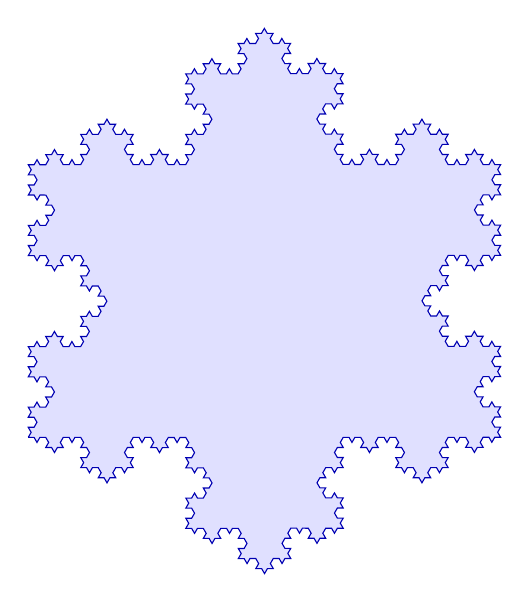
\begin{tikzpicture}[decoration=Koch snowflake]
  % Each decorate applies one more step; going round clockwise puts the bumps outside
  \filldraw[fill=blue!12, draw=blue!70!black, thin] decorate{ decorate{ decorate{ decorate{ (0,0) -- (60:6) -- (6,0) -- cycle }}}};
\end{tikzpicture}
